\documentclass{report}
\usepackage{graphicx}
\graphicspath{{./images/}}

\begin{document}
\title{Projet}
\maketitle
\newpage
\section{Diagrammes de séquence pour fournisseurs}
\subsection{Connection d'un fournisseur}

Lorsqu'un fournisseur veut se connecter, il doit entrer son identifiant et son mot de passe. Donc le cas où les informations sont correctes et qu'un fournisseur les possédant sont trouvé sur la base de données, la connection est réussie et le fournisseur se trouve sur sa page d'accueil. \\
Cependant, si au moins l'une des informations sont incorrectes, une message d'erreur sera affiché pour le fournisseur.
\\
\\
\begin{figure}[h]
	\centering
	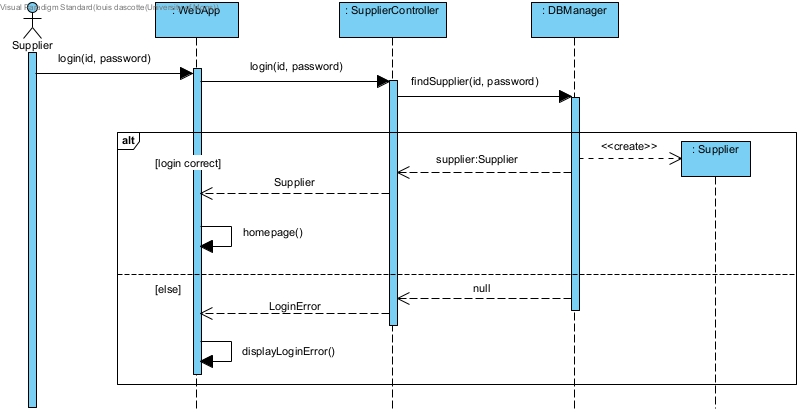
\includegraphics[width=1.3\textwidth]{Log In (Supplier)}
	\caption{Connection d'un fournisseur}
	\label{fig:login}
\end{figure}
\subsection{Importation des informations d'un compteur}

Un fournisseur peut importer des données depuis un fichier. Une fois les données extraites, on recherche si il existe un compteur correspondant. Si celui si existe, le controleur va vérifier si il y a des données en doublons sur certains jours. Si il y en a pas, l'importation continue normalement. Sinon, on a plusieurs options. \\
Le fournisseur peut soit écraser les données doublons et les remplacer par celles contenues dans le fichier. Il peut aussi ignorer les données en double du fichier et garder celle de base. Et pour finir l'importation peut être arrêtée.
\\
\\
\begin{figure}[h!]
    \centering
    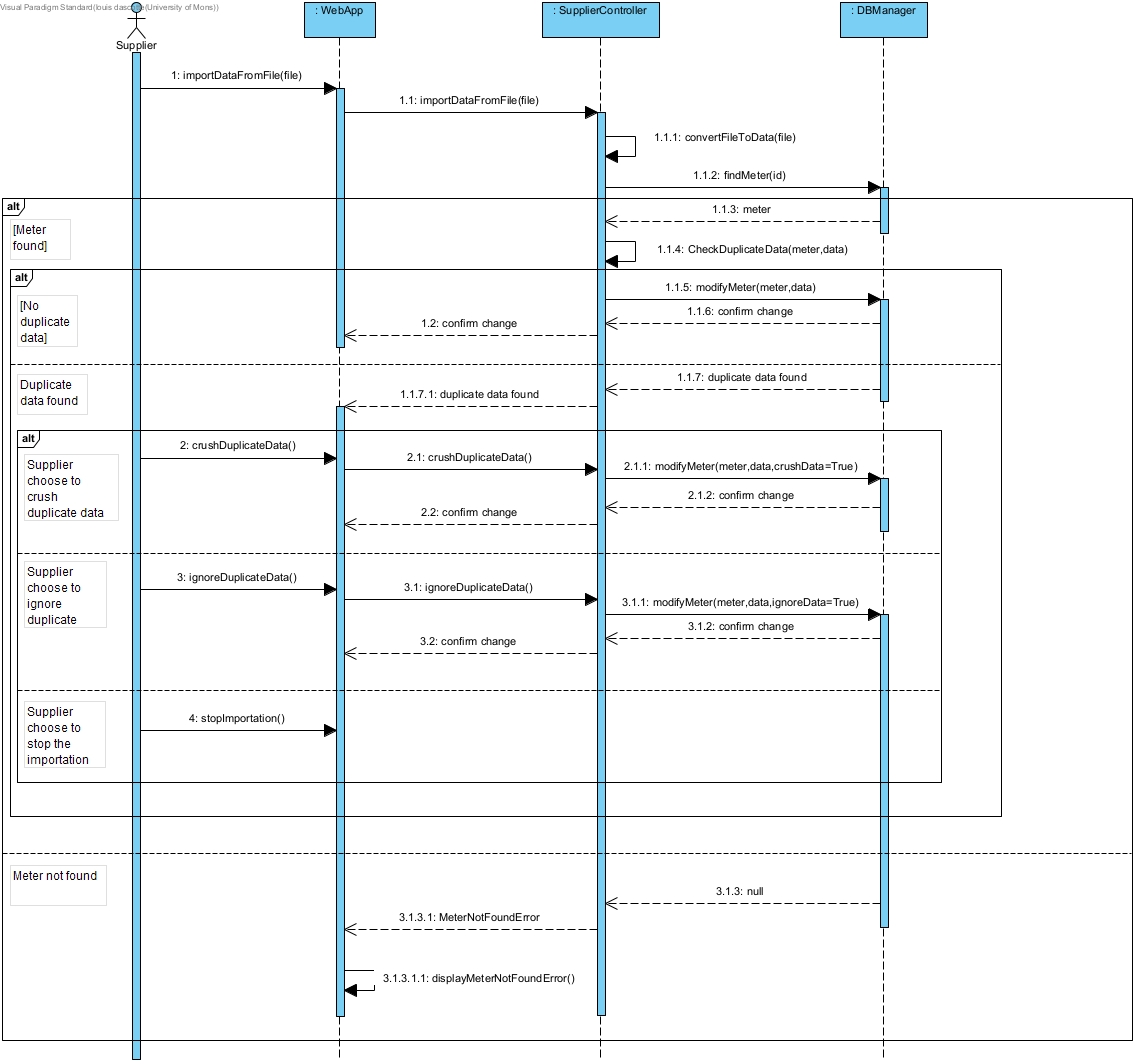
\includegraphics[width=1.3\textwidth]{Link consumption}
    \caption{Importation des informations d'un compteur}
    \label{fig:linkConsumption}
\end{figure}

\subsection{Remplir les requêtes}

Un fournisseur peut remplir les requêtes de ses clients et vérifier que les informations sur leurs compteurs soient correctes. \\
Par exemple, un client peut faire une demande de contrat, que le fournisseur verra dans ses notifications. Après, le fournisseur peut choisir soit de créer un nouveau contrat pour le client, soit le refuser. Dans les deux cas, le client sera notifié. \\
Ensuite, lorsque un client change les données d'un de ses compteurs, si besoin le fournisseur peut les changer si le client a mis des informations incorrectes, et le notifiera que les données du compteur ont changé.
\\
\\
\begin{figure}[h]
    \centering
    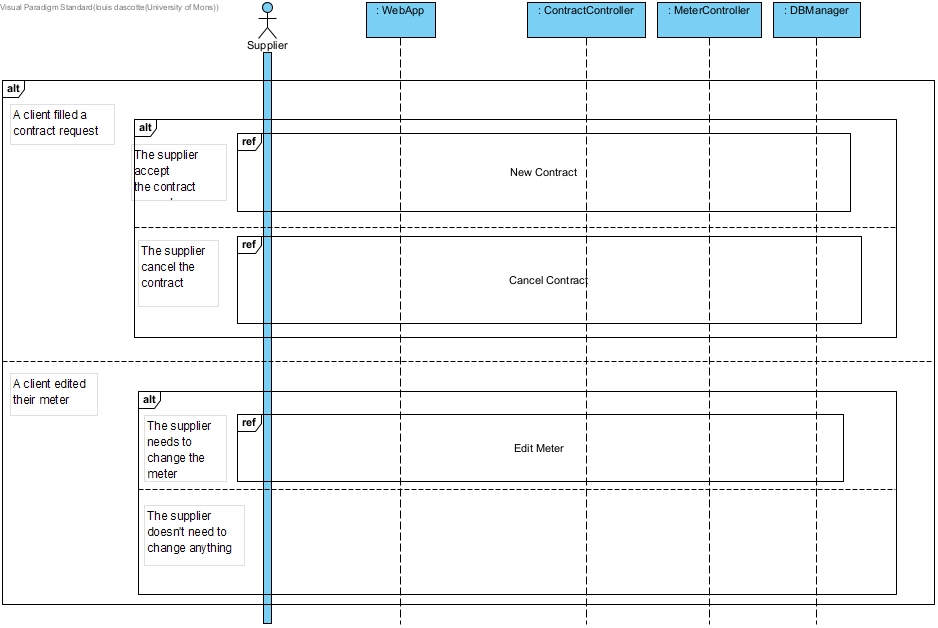
\includegraphics[width=1.3\textwidth]{process query}
    \caption{Remplir les requêtes}
    \label{fig:processQuery}
\end{figure}

\begin{figure}[h]
	\centering
	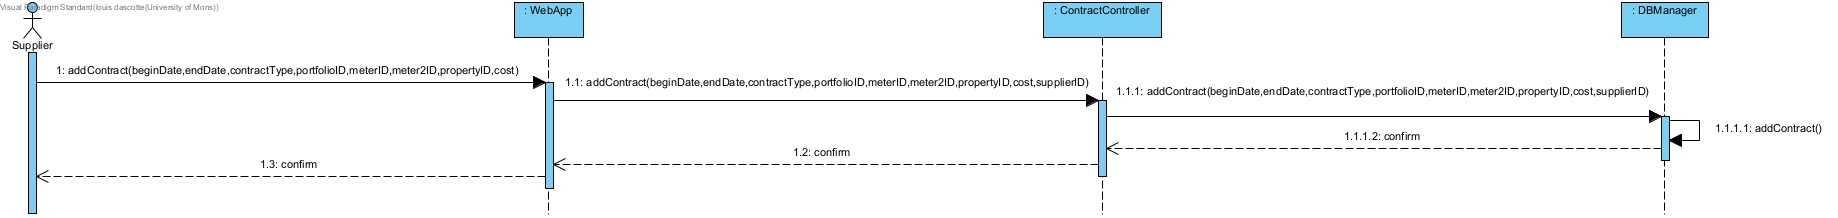
\includegraphics[width=1.3\textwidth]{New Contract}
	\caption{Création d'un nouveau contrat}
	\label{fig:newContract}
\end{figure}

\begin{figure}[h]
	\centering
	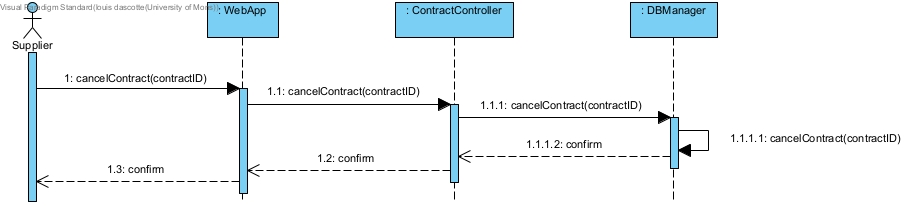
\includegraphics[width=1.3\textwidth]{Cancel Contract}
	\caption{Annulation du contrat}
	\label{fig:cancelContract}
\end{figure}

\begin{figure}[h]
	\centering
	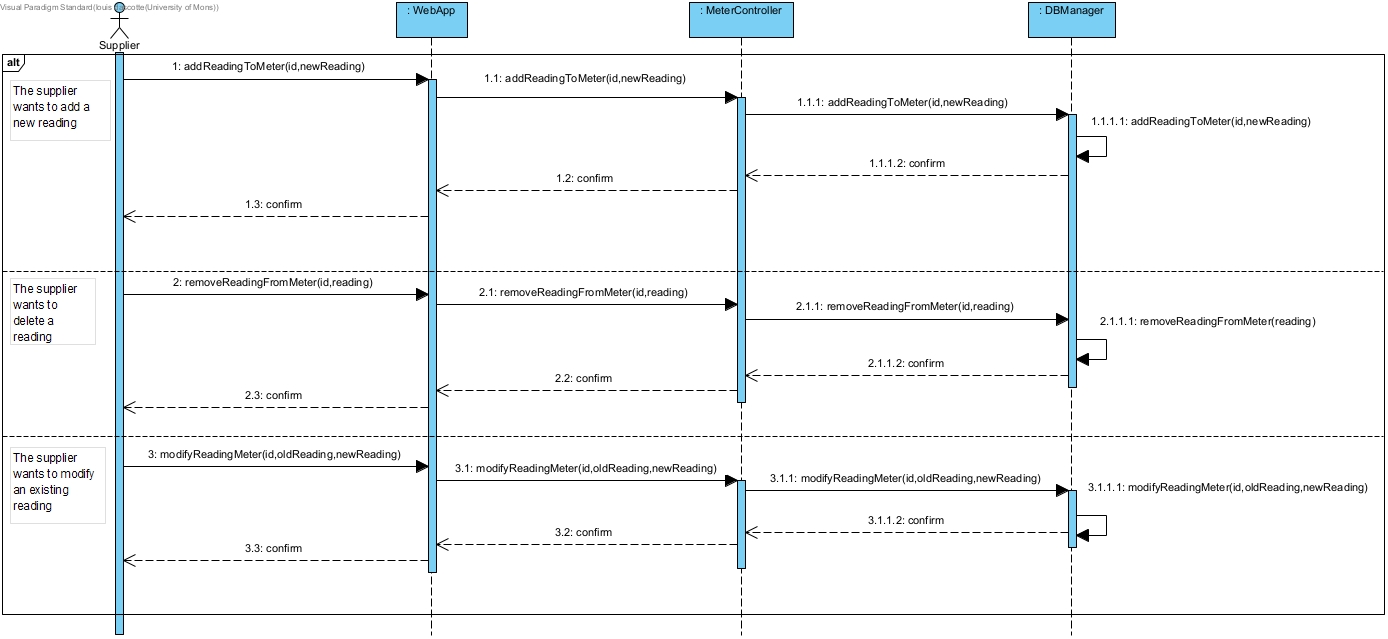
\includegraphics[width=1.3\textwidth]{Edit Meter}
	\caption{Modifier un contrat}
	\label{fig:cancelContract}
\end{figure}


\end{document}


